\documentclass[11pt]{article}

%Both greek and english language support
\usepackage[greek,english]{babel}
\usepackage[utf8]{inputenc}
\usepackage{alphabeta}

% For \includegraphics
\usepackage{graphicx}   
\usepackage[space]{grffile}

\usepackage{amsmath}
\usepackage[colorinlistoftodos]{todonotes}

% For hyper links
\usepackage[unicode]{hyperref}

%Diagonal line on Tables
\usepackage{diagbox}

%Multiple rows in tables
\usepackage{multirow}

% %----------------------------- MATLAB -----------------------------
\usepackage[T1]{fontenc}
% \usepackage{bigfoot} % to allow verbatim in footnote
\usepackage[numbered,framed]{matlab-prettifier}

\lstset{
  style              = Matlab-editor,
  basicstyle         = \mlttfamily,
  escapechar         = ",
  mlshowsectionrules = true,
}
\let\ph\mlplaceholder % shorter macro
\lstMakeShortInline"

% % In order to use Matlab code just use this 
% \begin{lstlisting}[caption = {Title}]
%   code
% \end{lstlisting}
% %----------------------------- MATLAB -----------------------------

%Convolution symbol
\usepackage{amssymb}

% Page margins 
\usepackage{geometry}
 \geometry{
 a4paper,
 total={170mm,257mm},
 left=20mm,
 top=20mm,
 }

\DeclareUnicodeCharacter{2212}{-}   %Negative exponential


\begin{document}
    %--------------------------------------------------------------------------------------------
    % Title Page
    \begin{titlepage}
        \center
        %----------------------------------------------------------------------------------------
        %	HEADING SECTIONS
        \textsc{\LARGE Technical University of Crete}\\[2cm] 
        \Large Τηλεπικοινωνιακά Συστήματα Ι\\[1cm] 
        
        \rule{\linewidth}{0.5mm} \\[0.5cm]
            { \huge \bfseries Άσκηση 1}\\[0.5cm]
        \rule{\linewidth}{0.5mm} \\[2.5cm]
        
        \begin{minipage}{0.4\textwidth}
            \begin{flushleft} \large
                \emph{Author:}\\
                    Σπυριδάκης Χρήστος
            \end{flushleft}
        \end{minipage}
        ~
        \begin{minipage}{0.4\textwidth}
            \begin{flushright} \large
                \emph{ΑΜ:} 2014030022
            \end{flushright}
        \end{minipage}\\[4cm]
        
        {\large October 31, 2019}\\[2cm] 
        %----------------------------------------------------------------------------------------
        %	LOGO
        
\includegraphics[scale=0.5]{TUC.png} 
        \vfill
    \end{titlepage}





    %-------------------------------------------------------------------------
    %   Eisagwgi
    \section{Εισαγωγή}
    Για την διευκόλυνση της υλοποίησης είναι καλό να σημειωθεί ότι το κάθε μέρος (Α, Β και C) υλοποιήθηκε σε διαφορετικό script, αυτό είχε τα θετικά του, στο να είναι περισσότερο διακριτός ο κώδικας για ανάπτυξη και αποσφαλμάτωση, αλλά χρειάστηκε να ξανά δημιουργηθούν σήματα που είχαν δημιουργηθεί σε προηγούμενα ερωτήματα. Δεν επηρεάζονται κάπως τα αποτελέσματα απλά είναι μία διευκρίνηση σχετικά με την δομή που δόθηκε στον κώδικα. 
    \par \noindent
    Επίσης τα πέντε σημαντικά αρχεία που υπάρχουν είναι το \emph{\texttt{srrc\_pulses.m}} το οποίο είναι αυτό που δόθηκε ως βοηθητικό αρχείο για την δημιουργία των αποκομμένων SRRC παλμών. Τα \emph{\texttt{part\_a.m}}, \emph{\texttt{part\_b.m}} και \emph{\texttt{part\_c.m}} τα οποία αναφέρονται για κάθε θέμα ξεχωριστά καθώς επίσης υπάρχει και το \emph{\texttt{bits\_to\_2PAM.m}} το οποίο εξηγείται περισσότερο στο θέμα C.
    \par \noindent
    Να αναφερθεί ότι στους ενδιάμεσους κώδικες (για το κάθε ερώτημα) εμφανίζεται ΜΟΝΟ το κομμάτι υπολογισμού του ερωτήματος, δεν εμφανίζονται δηλαδή κομμάτια κώδικα σχετικά με την δημιουργία των figure ή τις έξτρα πληροφορίες για αυτά, όπως επίσης και κάποια από τα σχόλια για εξοικονόμηση χώρου. Γενικά έχει ελαφρώς αλλαχθεί ο κώδικας που παρουσιάζεται σε κάθε ερώτηση ώστε να κρατηθούν μόνο τα σημαντικά σημεία. Στο τέλος της αναφοράς υπάρχει ολόκληρος ο κώδικας για έλεγχο και αυτών των σημείων.
    \par \noindent
    Τέλος, αν λόγω της εκτύπωσης σε χαρτί δεν είναι εμφανές σε ικανοποιητικό βαθμό κάποιο από τα figures μπορούν να βρεθούν όλα τα μέρη του project στο παρακάτω repository όπου υπάρχουν και screenshot αυτών που φαίνονται πιο λεπτομερειακά: \url{https://github.com/CSpyridakis/CommSys}



    %-------------------------------------------------------------------------
    %   A section
    \section{Ερώτημα Α}
    
    %-------------------------------------
    %   A.1 subsection
    \subsection*{Α.1 Δημιουργία των SRRC φ(t) παλμών}
    Αρχικά χρειάστηκε να χρησιμοποιήσουμε το script που μας δόθηκε - \emph{\texttt{srrc\_pulses.m}} - προκειμένου να δημιουργήσουμε αποκομμένους παλμούς Square Root Raised Cosine φ(t). Είσοδος της συνάρτησης είναι η περίοδος συμβόλων T, η περίοδος δειγματοληψίας Ts, ο θετικός αριθμός Α και το roll-off factor a. Όπου η περίοδος δειγματοληψίας υπολογίζεται ως το πηλίκο $\frac{T}{over}$, με over ως το συντελεστή υπερδειγματοληψίας. Στην περίπτωση μας για τα δεδομένα της εκφώνησης είχαμε $T = {10^{−2}}$ sec, $over = 10$, $A = 4$ και $a = 0, 0.5, 1$. Συνεπώς  δημιουργήθηκαν οι παρακάτω παλμοί:

    \begin{center}{}
        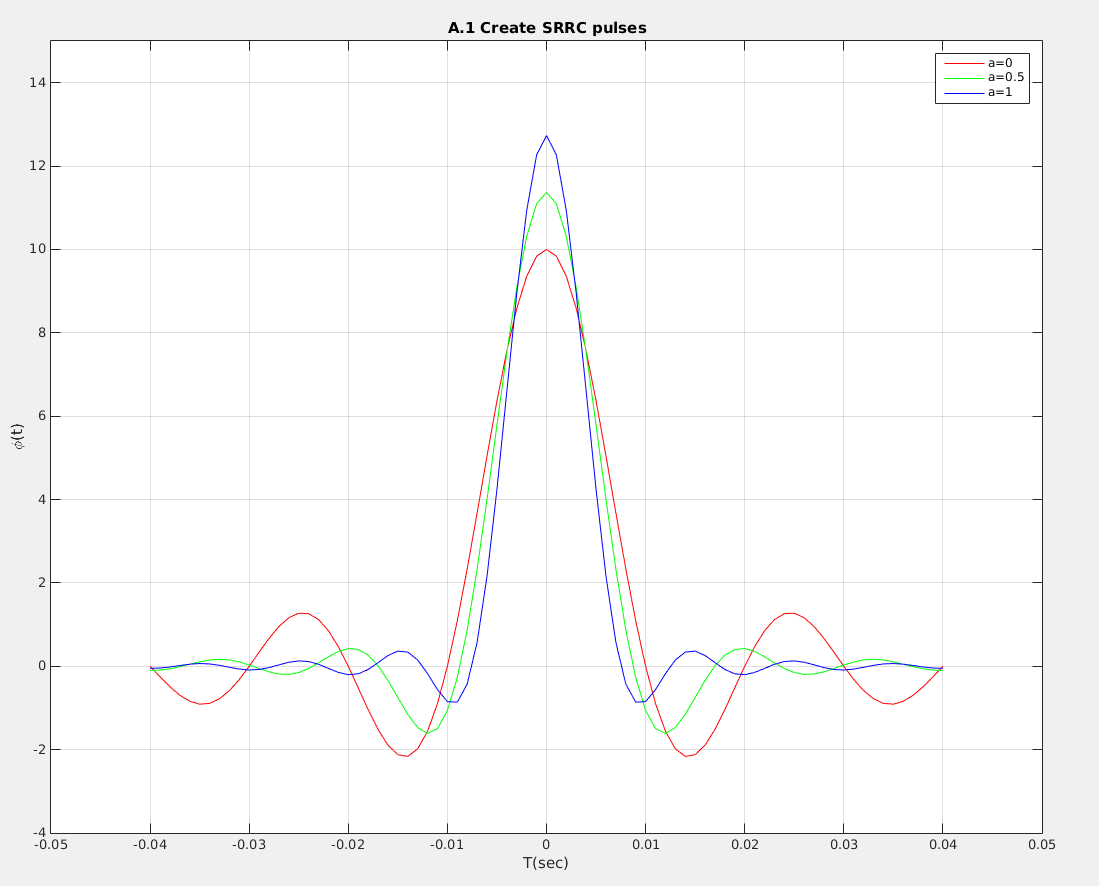
\includegraphics[scale=0.27]{photos/A.1 Create SRRC pulses_screenshot.png}
    \end{center}
    
    \par \noindent
    Αυτά που μπορούμε να παρατηρήσουμε και από τα διαγράμματα σχετικά με το ρυθμό “μείωσης” του πλάτους των παλμών είναι τα εξής. Πρώτη παρατήρηση είναι ότι για κάθε τιμή του roll-off γίνεται φθίνουσα ταλάντωση της οποία βέβαια τα χαρακτηριστικά εξαρτώνται από την τιμή του a. Επίσης, όλοι οι παλμοί έχουν την ίδια περίοδο. Ακόμα, βλέπουμε ότι για μεγαλύτερο a έχουμε και μεγαλύτερο αρχικό πλάτος, ενώ ταυτόχρονα όσο μεγαλύτερο είναι το a τόσο μεγαλύτερος είναι και ο ρυθμός απόσβεσης όσο αυξάνεται η απόλυτη τιμή του χρόνου.
    
\begin{lstlisting}[caption = {Α.1}]
T=10^-2 ; over=10 ; Ts=T/over ; A=4 ; a=[0 0.5 1] ; phi_t = [] ; t=[] ; 
f=figure();
for i=1:length(a)
  [phi_tmp t_tmp] = srrc_pulse(T, Ts, A, a(i));
  phi_t = [phi_t; phi_tmp];
  t = t_tmp;
  plot(t, phi_t(i,:), colors(i),'DisplayName',strcat('a=',num2str(a(i)))) ; hold on ; 
end
\end{lstlisting}
    
    %-------------------------------------
    %   A.2 subsection
    \subsection*{Α.2 Fourier Transform of SRRC pulses}
    Σε αυτό το ερώτημα ζητήθηκε να χρησιμοποιήσουμε τις συναρτήσεις fft και fftshift προκειμένου να υπολογίσουμε τον Fourier Transform των παλμών που μόλις δημιουργήσαμε και να σχεδιάσουμε την φασματική πυκνότητα ενέργειας αυτών. Αξίζει να γίνουν μερικές σημειώσεις σχετικά με την συγκεκριμένη υλοποίηση. Αρχικά το διάστημα συχνοτήτων του μετασχηματισμού, όπως δίνεται και από την εκφώνηση είναι το [−$\frac{F_s}{2}$, $\frac{F_s}{2}$). Για λόγους κανονικοποίησης έγινε πολλαπλασιασμός του fft result με το Ts ενώ επίσης, παρόλο που δεν ήταν απαραίτητο πραγματοποιήθηκε η ίδια διαδικασία για Νf (ισαπέχοντα σημεία) να ισούται με 1024 οσο και με 2048. Να αναφέρουμε ότι ο λόγος που χρησιμοποιείται το fftshift είναι για να μεταφέρει τον συντελεστή μηδενικής συχνότητας των παλμών στο κέντρο ώστε να μπορούν να συγκριθούν πιο εύκολα. Αφού είχαμε κάνει τα παραπάνω εμφανίζεται η ζητούμενη πληροφορία $|Φ(F)|^2$ τόσο σε κανονική κλίματα με την χρήση της συνάρτησης plot, όσο και σε ημι-λογαριθμική κλίμακα με την χρήση της συνάρτησης semilogy όπου μπορούμε να παρατηρήσουμε περισσότερες λεπτομέρειες, καθώς με αυτήν δίνεται η δυνατότητα να μελετήσουμε τις τιμές των $|Φ(F)|^2$ σε διαστήματα όπου αυτές είναι πολύ μικρές.
    
    
    \begin{center}
        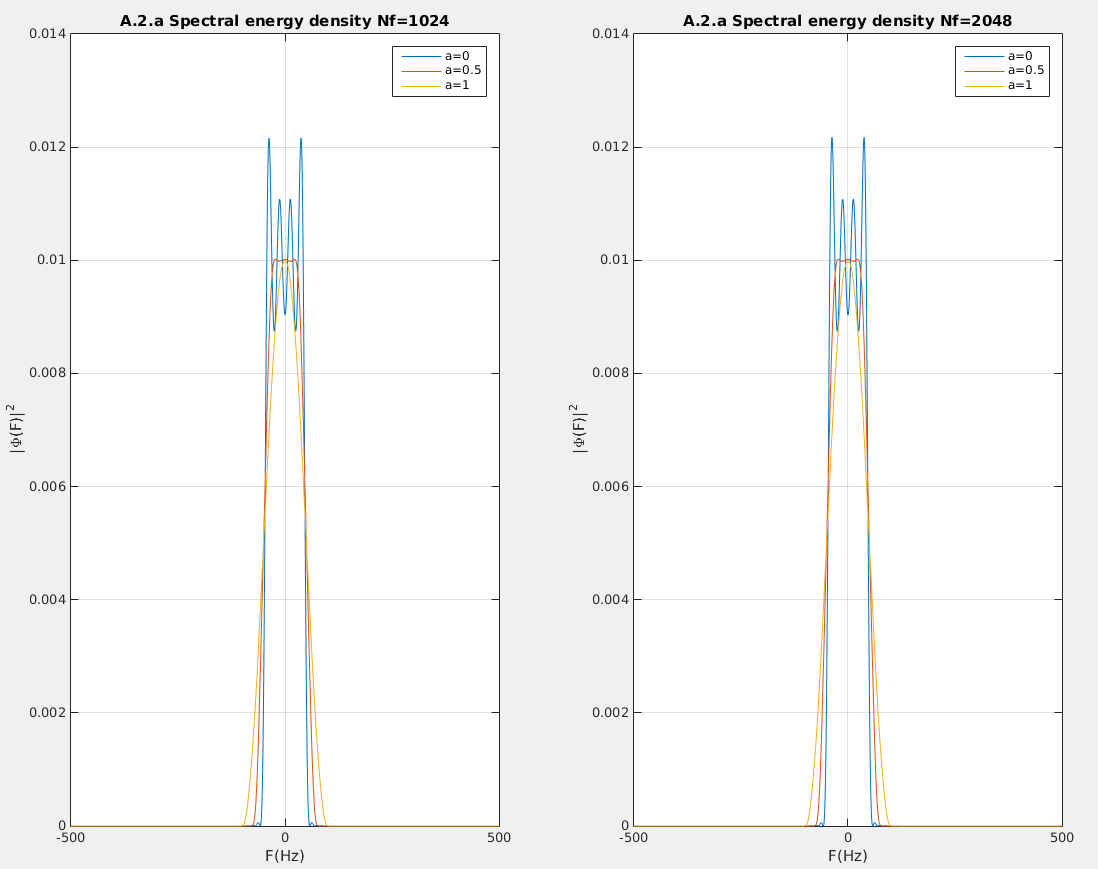
\includegraphics[scale=0.36]{photos/A.2 Fourier Transform phi(F)-Plots_screenshot.png}
    \end{center} 
    
    \begin{center}
        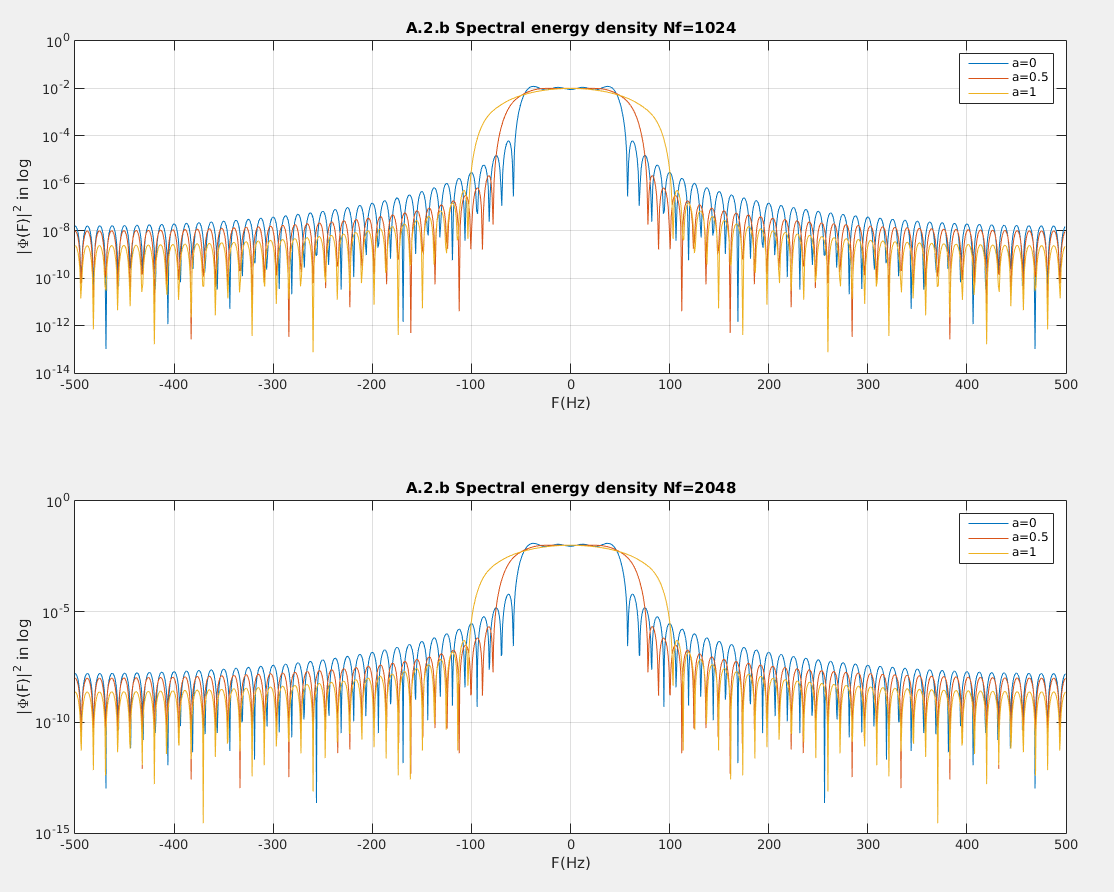
\includegraphics[scale=0.4]{photos/A.2 Fourier Transform phi(F)-Semilogy__screenshot.png}
    \end{center} 
    
\begin{lstlisting}[caption = {Α.2}]
Phi_F1 = [] ; Phi_F2 = [];
Fs = 1/Ts ; Nf = [1024 2048] ;              
F_1 = [-Fs/2 : Fs/Nf(1) : Fs/2-Fs/Nf(1)];  %Frequency vector Nf = 1024
F_2 = [-Fs/2 : Fs/Nf(2) : Fs/2-Fs/Nf(2)];  %Frequency vector Nf = 2048

for i=1:length(a)  %Fourier Transform
  X1 = fftshift(fft(phi_t(i,:),Nf(1))*Ts) ; Phi_F1 = [Phi_F1 ; X1] ;
  X2 = fftshift(fft(phi_t(i,:),Nf(2))*Ts) ; Phi_F2 = [Phi_F2 ; X2] ; 
end

f=figure();
subplot(1,2,1); % Nf = 1024 Plot
p1 = plot(F_1, abs(Phi_F1(1,:)).^2); hold on;
p2 = plot(F_1, abs(Phi_F1(2,:)).^2); hold on;
p3 = plot(F_1, abs(Phi_F1(3,:)).^2); hold off;
subplot(1,2,2); % Nf = 2048 Plot
p1 = plot(F_2, abs(Phi_F2(1,:)).^2); hold on;
p2 = plot(F_2, abs(Phi_F2(2,:)).^2); hold on;
p3 = plot(F_2, abs(Phi_F2(3,:)).^2); hold off;
...
f=figure(); extraInfo='-Semilogy';
subplot(2,1,1);  % Nf = 1024 Semilogy
p1 = semilogy(F_1, abs(Phi_F1(1,:)).^2); hold on;
p2 = semilogy(F_1, abs(Phi_F1(2,:)).^2); hold on;
p3 = semilogy(F_1, abs(Phi_F1(3,:)).^2); hold off;
subplot(2,1,2);  % Nf = 2048 Semilogy
p1 = semilogy(F_2, abs(Phi_F2(1,:)).^2); hold on;
p2 = semilogy(F_2, abs(Phi_F2(2,:)).^2); hold on;
p3 = semilogy(F_2, abs(Phi_F2(3,:)).^2); hold off;
\end{lstlisting}
    
    %-------------------------------------
    %   A.3 subsection
    \subsection*{Α.3 Bandwidth Calculation}
    Σκοπός του συγκεκριμένου ερωτήματος ήταν να δούμε τι συμβαίνει σχετικά με το εύρος φάσματος των παλμών, τόσο σε θεωρητικό όσο και σε πρακτικό επίπεδο - στο οποίο τότε θεωρητικά έχουν άπειρο - και κατά πόσο αυτό εξαρτάται από το συντελεστή roll-off a. Πρώτο βήμα ήταν να υπολογίσουμε τα θεωρητικά bandwidth για κάθε a μέσω του τύπου $BW = \frac{1+a}{2T}$. Αφού έγινε αυτό, υποθέσαμε μία νοητή ευθεία η οποία θα ήταν το πρώτο φράγμα των πειραμάτων, όπου χρησιμοποιήθηκε ως νοητό μηδέν. Σκοπός της ήταν να θεωρήσουμε ότι κάτω από αυτήν, οι παλμοί είναι πρακτικά μηδέν και σύμφωνα με αυτό να δούμε το πρακτικό BW. Μετά επαναλήφθηκε η ίδια διαδικασία για διαφορετική ευθεία προκειμένου να δούμε αν υπάρχουν διαφορετικά αποτελέσματα. Οι ευθείες που θεωρήσαμε ήταν η $C_1 = \frac{T}{10^3}$ και $C_2=\frac{T}{10^5}$ ενώ εμφανίζονται διαγράμματα και για τα δύο $N_f$ που δόθηκαν ως τυπικές τιμές.

    \begin{center}
        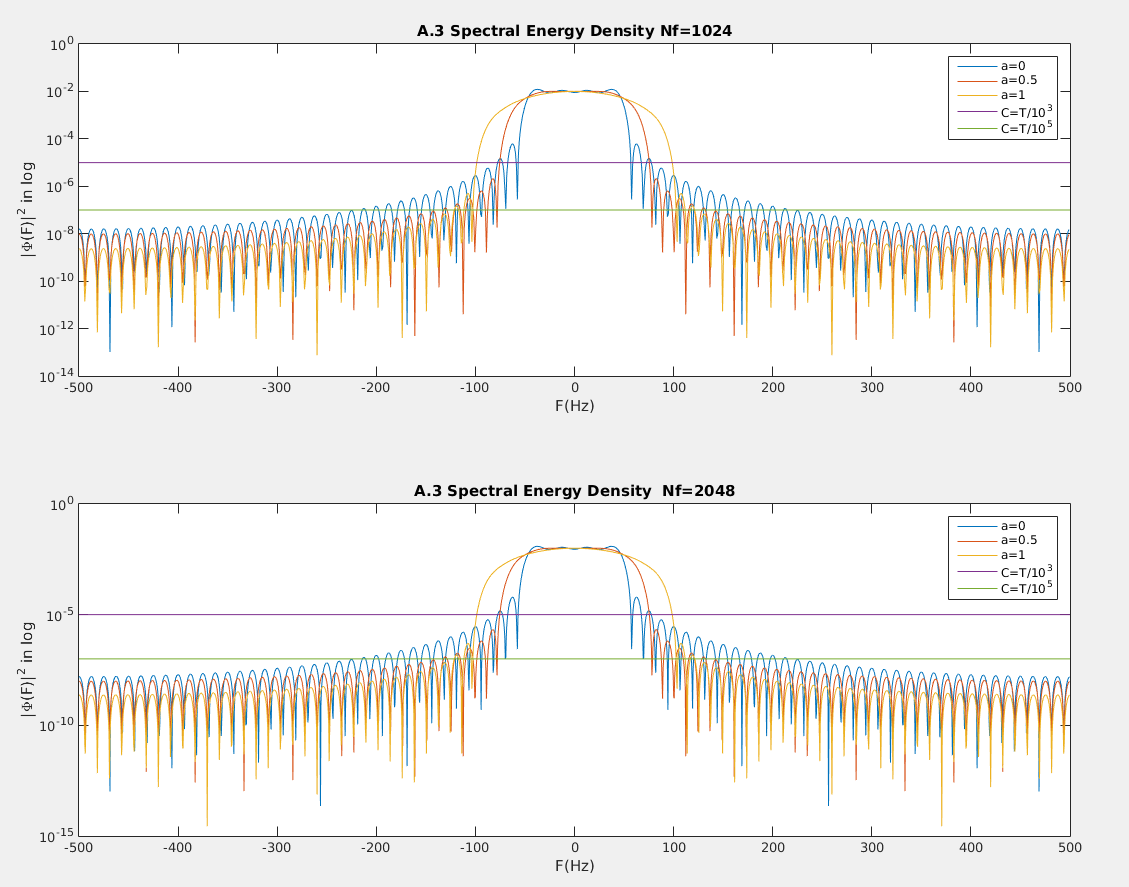
\includegraphics[scale=0.35]{photos/A.3 Bandwidth_screenshot.png}
    \end{center} 
    
    \par \noindent
    Προκειμένου να μπορέσουμε να διακρίνουμε προσεγγιστικά το εύρος φάσματος του κάθε παλμού μας βοήθησε η χρήση του zoom στα figures. Μαζί με το εργαλείο \emph{select data} για να βρούμε τις συντεταγμένες του άξονα x.
    
    \begin{center}
        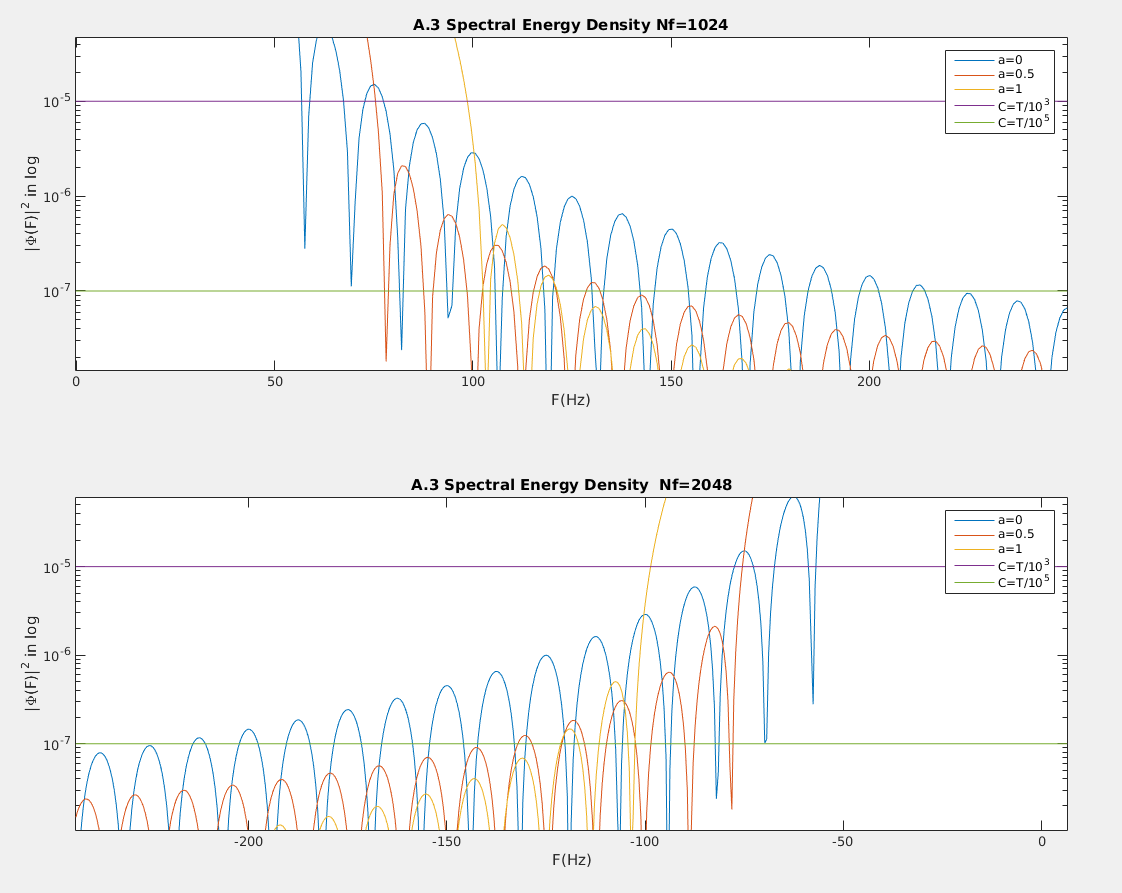
\includegraphics[scale=0.35]{photos/A.3 Bandwidth_screenshot_zoom.png}
    \end{center} 
    
    \par \noindent
    Σύμφωνα με τα παραπάνω δημιουργήθηκε ο παρακάτω πίνακας ο οποίος συνοψίζει όλες τις πληροφορίες.
    
    %Table for A.3
    \begin{center}
        \begin{tabular}{c|c|c c} 
            \multirow{2}{*}{\backslashbox{roll-off a}{BW}} & \multirow{2}{*}{Theoretical ($BW=\frac{1+a}{2T}$)} & \multicolumn{2}{c}{Practical} \\ \cline{3-4}
             &  & $c= \frac{T}{10^3}$ & $c= \frac{T}{10^5}$ \\[0.2cm] \hline
            0   & 50  & 77.6 & 214 \\ \hline
            0.5 & 75  & 75.5 & 132 \\ \hline
            1   & 100 & 98.6 & 121 \\ 
        \end{tabular}
    \end{center}
    
    \par \noindent
    Αυτό που μπορούμε να παρατηρήσουμε είναι ότι για  $c= \frac{T}{10^3}$  τότε πιο αποδοτικός παλμός (μικρότερος σε εύρος φάσματος) είναι αυτός με roll-off a=0.5 ενώ αντίθετα για $c= \frac{T}{10^5}$ είναι αυτός με a=1. Πράγμα που σημαίνει ότι στην πράξη δεν είναι μονοσήμαντα ορισμένο ποιος παλμός είναι βέλτιστος ως προς το εύρος φάσματος καθώς εξαρτάται από διάφορους παράγοντες όπως τη θεωρητική ευθεία που θα θεωρήσουμε ως “πρακτικά μηδέν”.
    
    
    %-------------------------------------------------------------------------
    %   B section
    \section{Ερώτημα B}
    Σε αυτό το θέμα της εργαστηριακής άσκησης χρειάστηκε να μελετήσουμε τους παλμούς που είχαμε ήδη δημιουργήσει SRRC φ(t) ως προς την ορθοκανονικότητα τους ως προς τις μετατοπίσεις τους κατά ακέραια πολλαπλάσια k της περιόδους τους Τ. Ξανά δημιουργήσαμε λοιπόν παλμούς SRRC φ(t) αυτή την φορά με Α=5 όπως ζητείται στην εκφώνηση.
    
    %-------------------------------------
    %   B.1.1 subsection
    \subsection*{B.1.1 Plot φ(t) and φ(t−kT)}
     Πρώτο ζητούμενο ήταν να σχεδιάσουμε σε κοινό plot τους παλμούς φ(t) και φ(t−kT) για a = 0, 0.5, 1 και k = 0, 1, 2, 4. Για να γίνει αυτό πρώτα έπρεπε να ορίσουμε κατάλληλα τον χρόνο ο οποίος εξαρτάται από τον αριθμό k, θυμόμαστε ότι κανονικά ο φ(t) ορίζεται στο $[-A*T, A*T]$ έπρεπε λοιπόν σε αυτό να προσθέσουμε τον έξτρα χρόνο για την μετατόπιση. Ενώ έπειτα για τα σήματα χρειάστηκε να κάνουμε zero padding όσα μηδενικά κάθε φορά έπρεπε σύμφωνα με την μετατόπιση που γινόταν. Για το φ(t) το zero padding θα γίνει προς τα δεξιά καθώς προς τα εκεί μετακινείται το άλλο σήμα ενώ για το φ(t−kT) προς τα αριστερά, αντίθετο δηλαδή με την φορά της κίνησης του. Τα σχήματα τα οποία δημιουργήθηκαν σύμφωνα με τα παραπάνω εμφανίζονται στα ακόλουθα διαγράμματα. 
     
\begin{lstlisting}[caption = {B.1.1}]
f=figure(); extraInfo=' Plot phi_t and phi_t_kT';
for i=1:length(a)             % for a = 0, 0.5, 1
 subplot(3,1,i) ; col=2;
 for k=[0 1 2 4]              % for k=0,1,2,4
  %Create signals
  t_s=[-A*T:Ts:(A+k)*T];    % time vector with needed extra time (A*T plus extra k*T)
  phi_t_za=[phi_t(i,:) zeros(1,k*over)];         % phi(t) (with zeros added)
  phi_kt_za=[zeros(1,k*over) phi_t(i,:)];        % phi(t-kT) (with zeros added)

  if k==0 % Plot once initial signal then plot others
   plot(t_s, phi_t_za, strcat(colors(1),'-'), 'DisplayName','\phi(t)') ; hold on ; 
   plot(t_s, phi_kt_za, strcat(colors(col),valueStyles(col)), 'DisplayName','\phi(t-kT), k=0') ; hold on ; col=col+1; 
  else
   plot(t_s, phi_kt_za, strcat(colors(col),'-',valueStyles(col)), 'DisplayName',strcat('\phi(t-kT), k=',num2str(k))) ; hold on ; col=col+1; 
  end
 end
end
\end{lstlisting}
    
    \begin{center}
        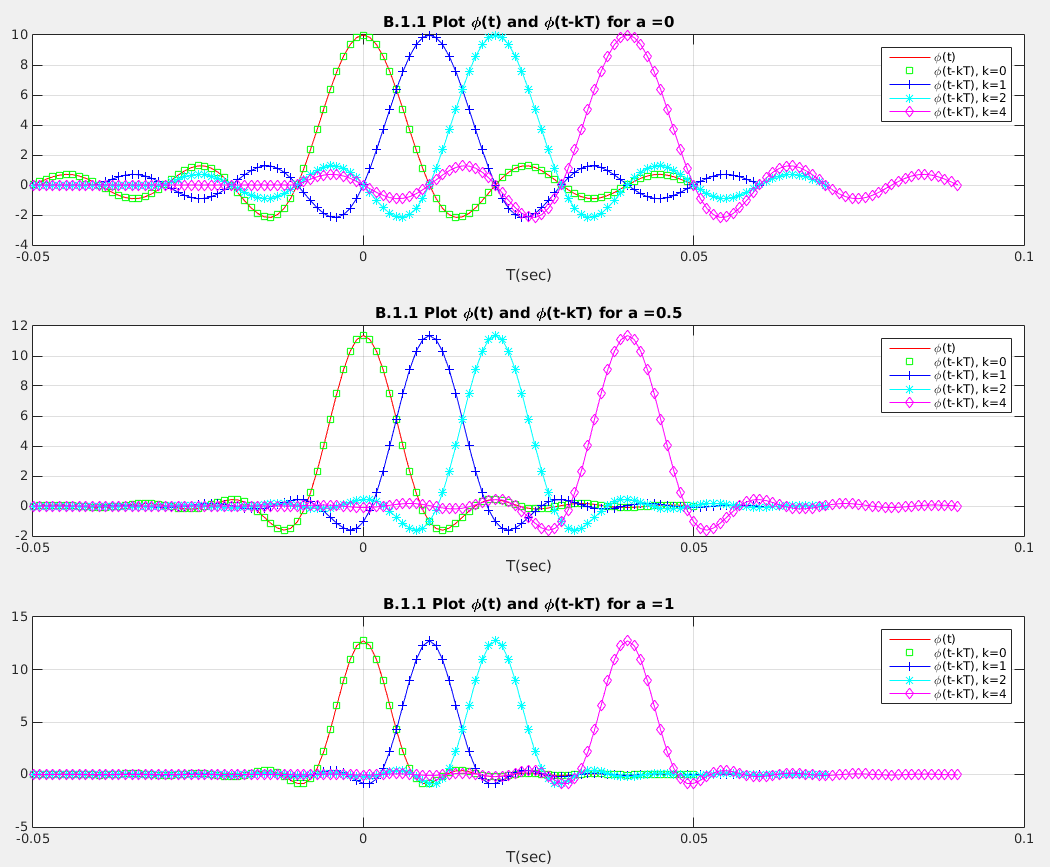
\includegraphics[scale=0.4]{photos/B.1.1 Plot phi_t and phi_t_kT_screenshot.png}
    \end{center} 
    
    %-------------------------------------
    %   B.1.2 subsection
    \subsection*{B.1.2 Plot φ(t)φ(t − kT)}
    Αφού είχαμε κάνει το παραπάνω υπολογίσαμε και σχεδιάσαμε τα γινόμενα φ(t) φ(t − kT ) για a = 0, 0.5, 1 και k = 0, 1, 2, 4 και παρακάτω εμφανίζονται τα αποτελέσματα που πήραμε.
    
    \begin{center}
        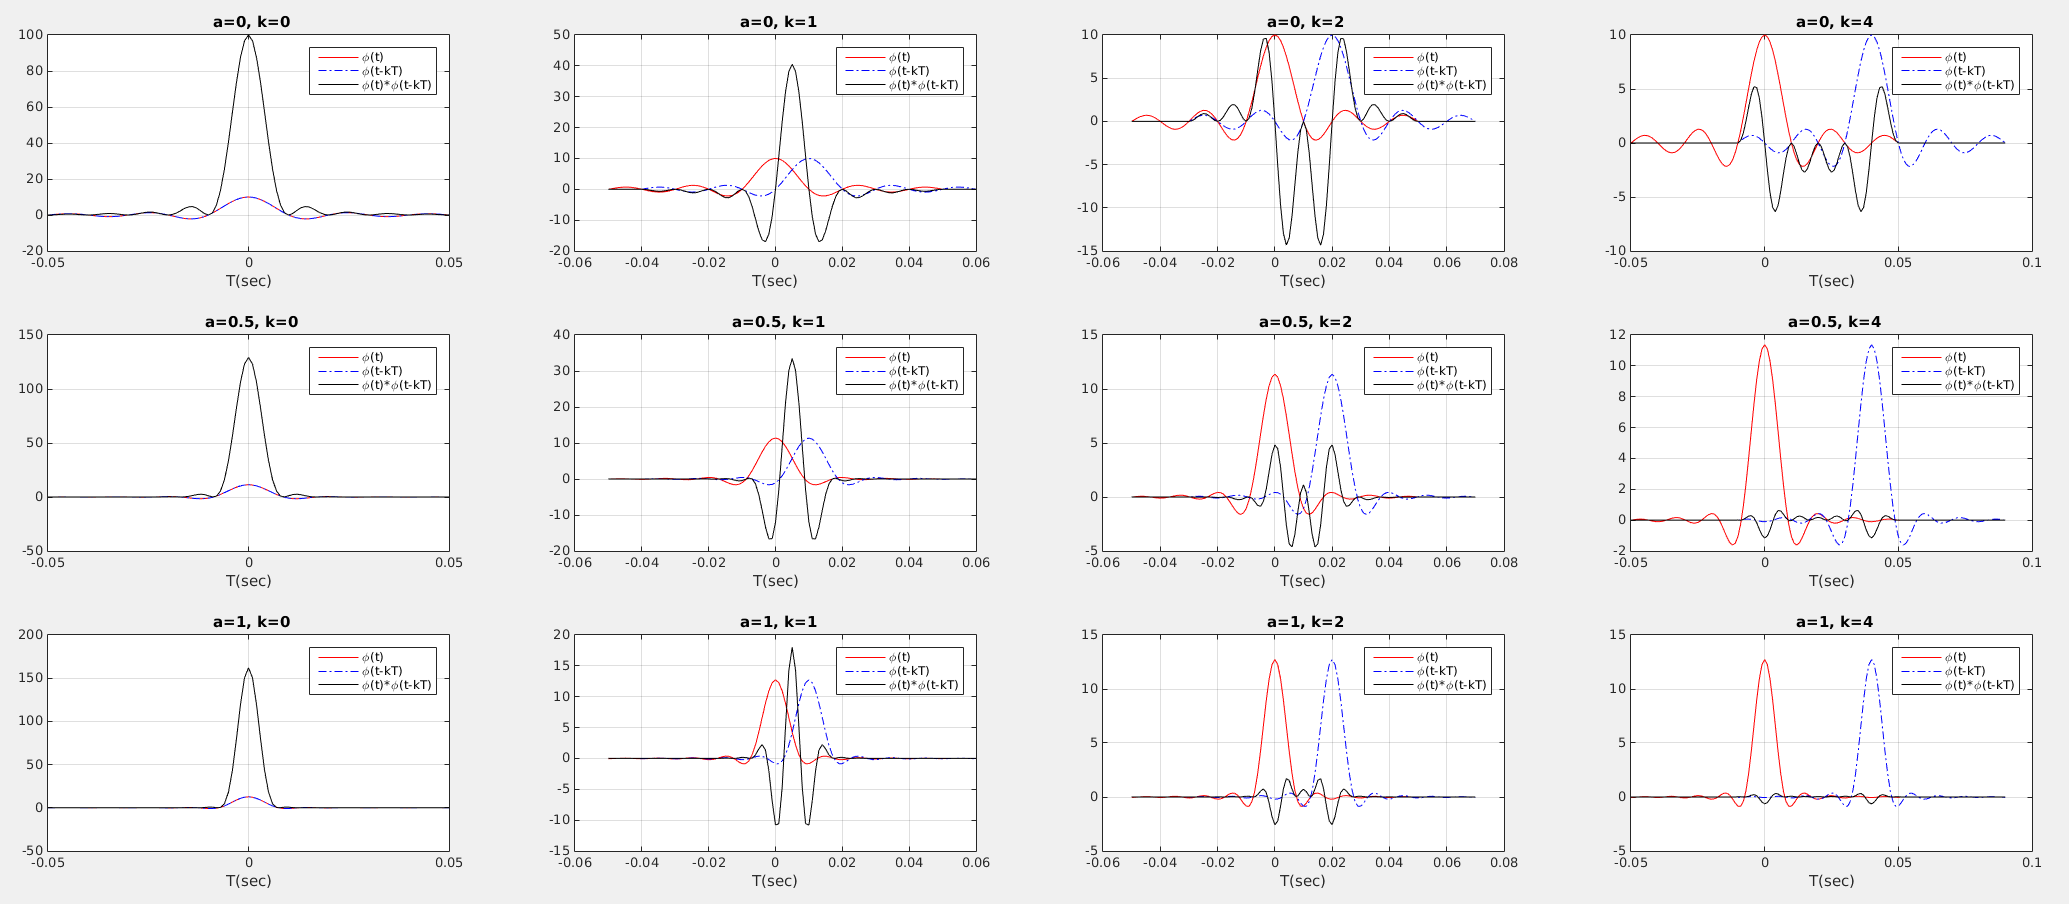
\includegraphics[scale=0.22]{photos/B.1.2 Products_screenshot_with_black.png}
    \end{center} 
    
\begin{lstlisting}[caption = {B.1.2}]
for i=1:length(a)             % for a = 0, 0.5, 1
 for k=[0 1 2 4]              % for k = 0,1,2,4
  subplot(3,4,p_num) ; p_num=p_num+1 ; col=2;
  %Create signals again
  t_s=[-A*T:Ts:(A+k)*T];    % time vector with needed extra time (A*T plus extra k*T)
  phi_t_za=[phi_t(i,:) zeros(1,k*over)];    % phi(t) (with zeros added)
  phi_kt_za=[zeros(1,k*over) phi_t(i,:)];   % phi(t-kT) (with zeros added)
  
  plot(t_s, phi_t_za, 'r-', 'DisplayName','\phi(t)') ; hold on ;   % phi(t) 
  plot(t_s, phi_kt_za, 'b-.', 'DisplayName', '\phi(t-kT)') ; hold on ;   % phi(t-kT)
  plot(t_s, phi_t_za.*phi_kt_za,'g', 'DisplayName','\phi(t)*\phi(t-kT)') ; hold off;    % phi(t)*phi(t-kT) 
 end
end
\end{lstlisting}
    
    %-------------------------------------
    %   B.1.3 subsection
    \subsection*{B.1.3 Calculate $\int_{}^{} φ(t)φ(t − kT) dt$}
    Αφού κάναμε αυτά προσεγγίσαμε αριθμητικά το ολοκλήρωμα του γινομένου φ(t) φ(t−kT) για
    a = 0, 0.5, 1 και k = 0, 2, 4. Ο τρόπος με τον οποίο το κάναμε ήταν ουσιαστικά με το να αθροίσουμε τις τιμές για τα γινόμενα που ήδη έχουμε υπολογίσει. Παρακάτω παρατίθεται ο πίνακας με τις τιμές των integrals που ζητήθηκαν.
    
    %Table for B.3
    \begin{center}
        \begin{tabular}{c|c|c|c}
            \backslashbox{a}{k} & 0 & 2 & 4 \\ \hline
            0   & 0.9798 & -0.0258 & -0.0402 \\ \hline
            0.5 & 0.9999 & 0.0002  & -0.0009 \\ \hline
            1   & 1.0000 & -0.0000 & -0.0001 \\
        \end{tabular}
    \end{center}
    
    \par \noindent
    Όπως μπορούμε να παρατηρήσουμε και από τον πίνακα μπορούμε να δούμε ότι οι αποκομμένοι SRRC παλμοί είναι προσεγγιστικά ορθοκανονικοί, ως προς τις μετατοπίσεις τους
    κατά kT καθώς για $k=0$ και οι τρεις περιπτώσεις ισούνται σχεδόν με την μονάδα ενώ για $k\neq0$ πλησιάζουν το 0 με την προσέγγιση να βελτιώνεται όσο το a πλησιάζει τη μονάδα. 

\begin{lstlisting}[caption = {B.1.3}]
for i=1:length(a)
  for k=[0 2 4]
    %Create signals again without time vector
    phi_t_za=[phi_t(i,:) zeros(1,k*over)];         % phi(t) (with zeros added)
    phi_kt_za=[zeros(1,k*over) phi_t(i,:)];        % phi(t-kT) (with zeros added)
  
    integrals=[integrals sprintf('a=%.1f, k=%d, integral=%.4f\n',a(i),k,sum(phi_t_za.*phi_kt_za)*Ts)];
  end
end
\end{lstlisting}

    %-------------------------------------------------------------------------
    %   C section
    \section{Ερώτημα C}
    Σε αυτό το ζητούμενο είχαμε να προσομοιώσουμε ένα 2-PAM σύστημα βασικής ζώνης το οποίο μεταφέρει N bits. Αρχικά δημιουργήσαμε ένα SRRC παλμό με χαρακτηριστικά $T=0.1$ sec, $over=10$, $a=0.5$, και $A=5$.
    
    %-------------------------------------
    %   C.1 subsection
    \subsection*{C.1 Δημιουργία N bits}
    Πρώτο πράγμα που μας ζητήθηκε ήταν να δημιουργήσουμε τα Ν bits, σε αυτή την υλοποίηση επιλέχθηκε $Ν = 100$. Ο τρόπος με τον οποίο δημιουργήθηκαν ήταν με την χρήση της σύνθετης εντολής: 
    
    $$b = (sign(randn(N, 1)) + 1)/2;$$
    
    \par \noindent
    Όπου πρώτα υπάρχει η χρήση της $randn(N,1)$ ώστε να δημιουργήσουμε ένα πίνακα Nx1 από αριθμούς κανονικής κατανομής έπειτα με την χρήση της sign κρατάμε το πρόσημο του κάθε αριθμού πολλαπλασιασμένο με την μονάδα άρα μέχρι αυτό το σημείο έχουμε ένα πίνακα με -1 και 1, στην συνέχεια προσθέτουμε σε αυτούς την μονάδα για να δημιουργήσουμε ένα πίνακα με στοιχεία 0 και 2 και προκειμένου να δημιουργήσουμε τελικά τον πίνακα από bits διαιρούμε αυτά τα στοιχεία με το 2 ώστε να πάρουμε 0 και 1.


    %-------------------------------------
    %   C.2.a subsection
    \subsection*{C.2.a 2-PAM διαμόρφωση βασικής ζώνης}
    Πλέον σκοπός ήταν να κωδικοποιήσουμε τα bits που μόλις δημιουργήσαμε σε 2-PAM βασικής ζώνης. Για να το κάνουμε αυτό δημιουργήθηκε το script: \texttt{bits\_to\_2PAM(b)} το οποίο παίρνει ως όρισμα ένα πίνακα b - ακολουθία bits - Νx1 στοιχείων και μέσω απλών συνθηκών μετασχηματίζει σύμφωνα με την εκφώνηση το 0 σε +1 και 1 σε -1. Δηλαδή επιστρέφει την ακολουθία από 2-PAM σύμβολα X.
    
\begin{lstlisting}[caption = {\texttt{bits\_to\_2PAM.m}}]
function [ Xo ] = bits_to_2PAM( Xi )
    Xo=zeros(1,length(Xi));    
    for i=1:length(Xi)    
        if(Xi(i)>0)          
            Xo(i)=-1;        
        else
            Xo(i)=1;    
        end
    end
end
\end{lstlisting}
    
    
    %-------------------------------------
    %   C.2.b subsection
    \subsection*{C.2.b Δημιουργία $X_δ(t)$}
    Αφού είχαμε δημιουργήσει το 2-PAM βασικής ζώνης χρησιμοποιούμε την upsample η οποία αυξάνει το ρυθμό δειγματοληψίας του σήματος Χ προσθέτοντας ανάμεσα στα δείγματα over-1 μηδενικά. Αυτό που θέλαμε να πετύχουμε είναι να προσωμοιώσουμε το σήμα $X_δ(t)$ μέσω της εντολής 
    $$\texttt{X\_delta} = 1/T s * upsample(X, over);$$
    Ό υπολογισμός του σήματος $X_δ$ ήταν εύκολος, αυτό που έπρεπε όμως να κάνουμε έξτρα ήταν να ορίσουμε κατάλληλα τον άξονα του χρόνου και να το σχεδιάσουμε. Σύμφωνα με τα παραπάνω ο χρόνος θα έπρεπε να είναι:
    $$\texttt{t\_delta} = [ 0 : Ts : (N*over-1)*Ts ];$$

    \begin{center}
        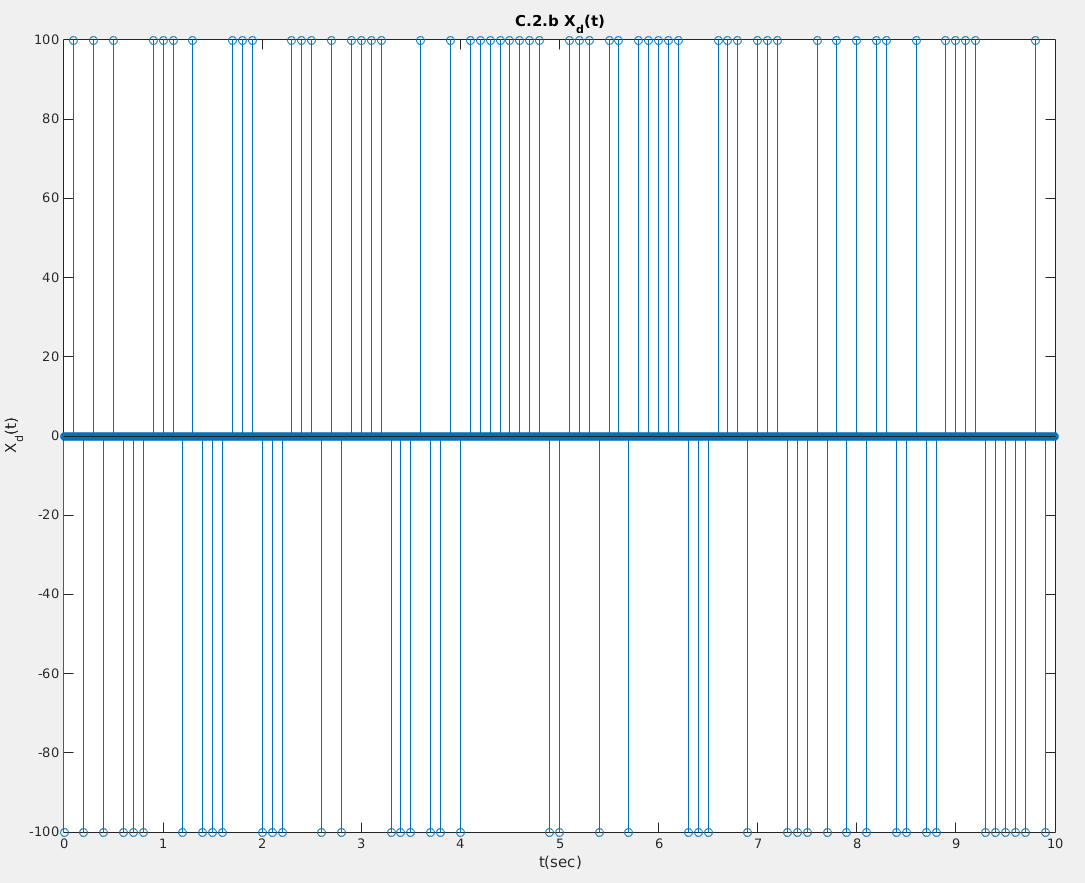
\includegraphics[scale=0.35]{photos/C.2.b X_d(t)_screenshot.png}
    \end{center} 
    
    %-------------------------------------
    %   C.2.c subsection
    \subsection*{C.2.c Δημιουργία $X(t)$}
    Προκειμένου να υπολογίσουμε την συνέλιξη του $X(t) = X_δ (t) \circledast  φ(t)$. Χρησιμοποιήσαμε την έτοιμη συνάρτηση του MATLAB και κανονικοποιήσαμε πολλαπλασιάζοντας με το Ts αφού μιλάμε για αναλογική συνέλιξη, ενώ όπως αναφέρεται και στην εκφώνηση για τον ορισμό του άξονα του χρόνου δεν είχαμε παρά να αθροίσουμε τα όρια των δύο σημάτων. Παρακάτω παρουσιάζεται η ζητούμενη συνέλιξη.
    
    \begin{center}
        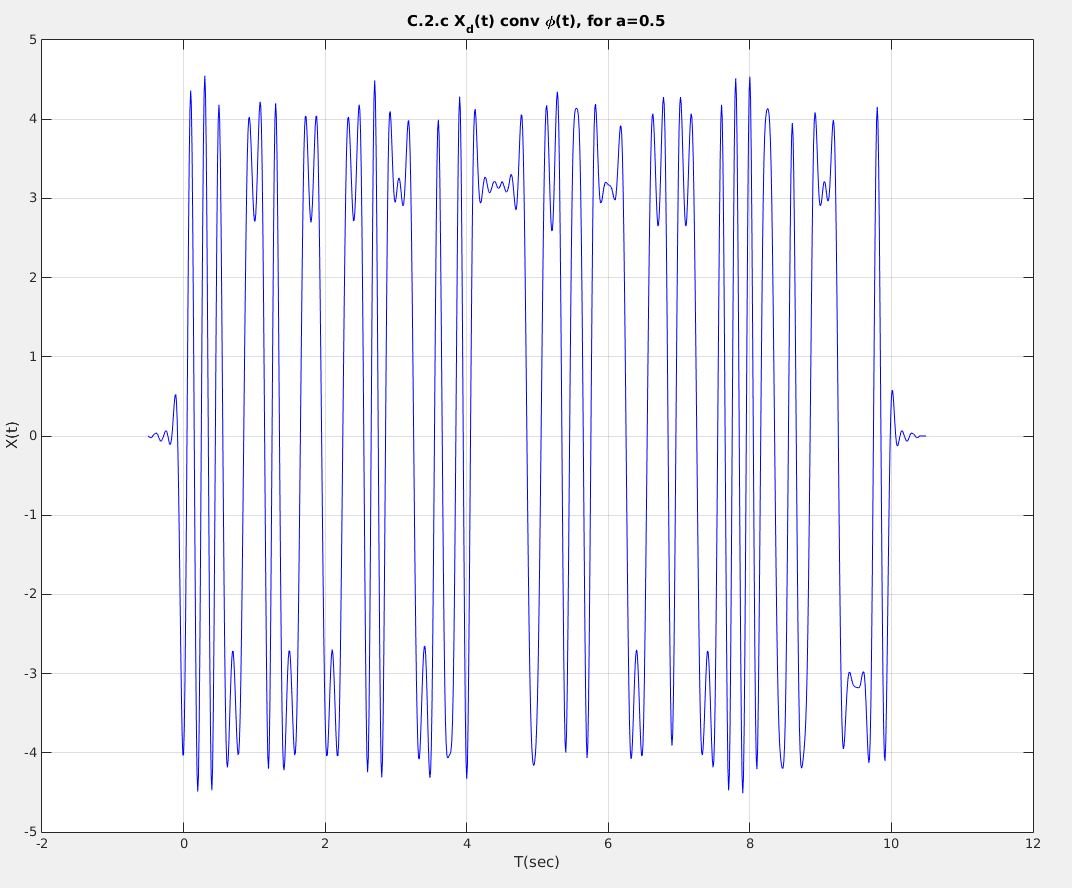
\includegraphics[scale=0.35]{photos/C.2.c X(t)_screenshot.png}
    \end{center} 

\begin{lstlisting}[caption = {C.2.c}]
[phi t_phi] = srrc_pulse(T, Ts, A, a); % Create SRRC pulse for this part

t_Xd_conv_phi = [t_delta(1) + t_phi(1) : Ts : t_delta(end) + t_phi(end)]; %time vector
X_t=conv(X_delta,phi)*Ts;   % Convolution

f=figure();
plot(t_Xd_conv_phi, X_t, 'b') ; grid on;  %Plot Xd(t) ** phi(t)
\end{lstlisting}

    %-------------------------------------
    %   C.2.d subsection
    \subsection*{C.2.d Δημιουργία $Z(t)$}
    Τέλος το μόνο που είχαμε να κάνουμε είναι να υποθέσουμε ιδανικό κανάλι και να υπολογίσουμε το αποτέλεσμα του δέκτη. Το οποίο ουσιαστικά είναι η συνέλιξη $Z(t) = X(t) \circledast φ(−t)$. Ακολουθήθηκε παρόμοια διαδικασία με το ερώτημα C.2.c με την διαφορά ότι έπρεπε να ανακλάσουμε το σήμα φ(t). Στο ίδιο σχεδιάγραμμα εμφανίζουμε και τις τιμές του $X_k$ , για k = 0, . . . , N − 1 που είναι ουσιαστικά τα σύμβολα που δημιουργήσαμε στον πομπό. Αυτό που παρατηρούμε είναι ότι οι τιμές της δειγματοληψίας συμπίπτουν με ικανοποιητική ακρίβεια με τον παλμό μας. Άρα μπορούμε να ανακτήσουμε πλήρως την αρχική πληροφορία αφού το φ(t) είναι ορθοκανονική όπως είδαμε παραπάνω.
    
    \begin{center}
        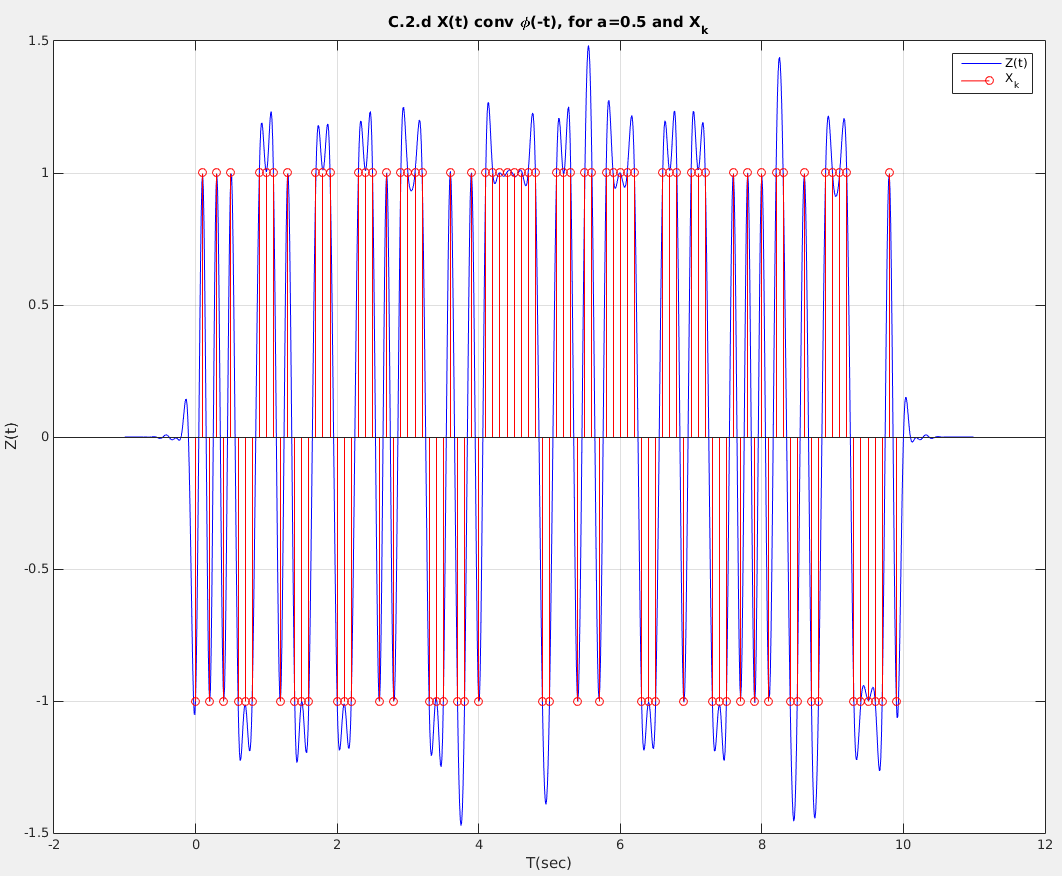
\includegraphics[scale=0.4]{photos/C.2.d Z(t) and Xk_screenshot.png}
    \end{center} 

\begin{lstlisting}[caption = {C.2.d}]
phi_rev = phi(end:-1:1); t_phi_rev = t_phi; % Revert phi(t) to create phi(-t)

t_Xd_conv_phi_rev = [t_Xd_conv_phi(1) + t_phi_rev(1) : Ts : t_Xd_conv_phi(end) + t_phi_rev(end)];
Z_t=conv(X_t,phi_rev)*Ts; % Convolution

f=figure();
p1 = plot(t_Xd_conv_phi_rev, Z_t, 'b') ; hold on; % Plot Xd(t) ** phi(-t)
p2 = stem([0:N-1]*T, X,'r') ; hold off;           % Stem Xk 
\end{lstlisting}

%---------------------------------------------------------------------------------------------------------------
%
%   Codes
%
%
\newpage

\begin{lstlisting}[caption = {\texttt{bits\_to\_2PAM.m}}]
function [ Xo ] = bits_to_2PAM( Xi )
    Xo=zeros(1,length(Xi));    
    for i=1:length(Xi)    
        if(Xi(i)>0)          
            Xo(i)=-1;        
        else
            Xo(i)=1;    
        end
    end
end
\end{lstlisting}

%%%%%%%%%%%%%%%%%%%%%%%%%%%%%%%%%%
%
%       Part a code
%
%
\begin{lstlisting}[caption = {\texttt{part\_a.m}}]
% ---------------------------------------------------------------------------------
%   Exercise 1, part A
%
%   Authors : Spyridakis Christos
%   Created Date : 26/10/2019
%   Last Updated : 30/10/2019
%
%   Description: 
%               Code created for Exercises of Communication Systems Course
%               in Tecnhical University of Crete
% ---------------------------------------------------------------------------------

clear all ; close all ; clc ;

% Just for saving in a separate folder figures as images
DEBUG = true ; part = 'A.' ;dirpath = '../doc/photos' ; ext = '.jpg' ; if ~DEBUG && ~exist(dirpath,'dir') ; mkdir(dirpath); end
% Auxiliary variables for plots, semilogy, etc...
colors = ['r' 'g' 'b' 'c' 'm' 'y' 'k'] ;
valueStyles = ['o' 's' '+' '*' 'd' '.' 'x' ];

%%%%%%%%%%%%%%%%%%%%%%%%%%%%%%%%%%%%%%%%%%%%%%%%%%%
% A.1
%
% Init mantatory variables
stepName = '1 Create SRRC pulses'; extraInfo = '';
T=10^-2 ; over=10 ; Ts=T/over ; A=4 ; a=[0 0.5 1] ; phi_t = [] ; t=[] ; 

% Create srrc pulses and plot them 
f=figure();
  for i=1:length(a)
    [phi_tmp t_tmp] = srrc_pulse(T, Ts, A, a(i));
    phi_t = [phi_t; phi_tmp];
    t = t_tmp;
    
    % Plot each srrc with a color and save plot to add extra info later  
    plot(t, phi_t(i,:), colors(i),'DisplayName',strcat('a=',num2str(a(i)))) ; hold on ; 
  end
  hold off ; axis([-0.05 0.05 -4 15]) ;

  % Add more info to plots                                           
  legend('Location','NorthEast');  grid on;
  title(strcat(part,stepName)); ylabel('\phi(t)'); xlabel('T(sec)');  
if ~DEBUG ; saveas(f,strcat(dirpath, '/', part, stepName, extraInfo, ext)) ; end 

%%%%%%%%%%%%%%%%%%%%%%%%%%%%%%%%%%%%%%%%%%%%%%%%%%%
% A.2
%
% Init mantatory variable 
stepName = '2 Fourier Transform phi(F)';
Phi_F1 = [] ; Phi_F2 = [];

% Calculate frequency vectors
Fs = 1/Ts ; Nf = [1024 2048] ;              
F_1 = [-Fs/2 : Fs/Nf(1) : Fs/2-Fs/Nf(1)];   % Frequency vector for Nf=1024
F_2 = [-Fs/2 : Fs/Nf(2) : Fs/2-Fs/Nf(2)];   % Frequency vector for Nf=2048

%Fourier Transform and save to vector
for i=1:length(a)
  X1 = fftshift(fft(phi_t(i,:),Nf(1))*Ts) ; Phi_F1 = [Phi_F1 ; X1] ;
  X2 = fftshift(fft(phi_t(i,:),Nf(2))*Ts) ; Phi_F2 = [Phi_F2 ; X2] ; 
end

% Plot them 
f=figure();  extraInfo='-Plots';
  % Nf = 1024
  subplot(1,2,1); 
  p1 = plot(F_1, abs(Phi_F1(1,:)).^2); hold on;
  p2 = plot(F_1, abs(Phi_F1(2,:)).^2); hold on;
  p3 = plot(F_1, abs(Phi_F1(3,:)).^2); hold off;
  legend([p1,p2,p3],'a=0', 'a=0.5', 'a=1'); legend('Location','NorthEast'); grid on;
  title('A.2.a Spectral energy density Nf=1024'); ylabel('|\Phi(F)|^2'); xlabel('F(Hz)');
  % Nf = 2048
  subplot(1,2,2); 
  p1 = plot(F_2, abs(Phi_F2(1,:)).^2); hold on;
  p2 = plot(F_2, abs(Phi_F2(2,:)).^2); hold on;
  p3 = plot(F_2, abs(Phi_F2(3,:)).^2); hold off;
  legend([p1,p2,p3],'a=0', 'a=0.5', 'a=1'); legend('Location','NorthEast'); grid on;
  title('A.2.a Spectral energy density Nf=2048'); ylabel('|\Phi(F)|^2'); xlabel('F(Hz)');
if ~DEBUG ; saveas(f,strcat(dirpath, '/', part, stepName, extraInfo, ext)) ; end

% Semilogy 
f=figure(); extraInfo='-Semilogy';
   % Nf = 1024
  subplot(2,1,1); 
  p1 = semilogy(F_1, abs(Phi_F1(1,:)).^2); hold on;
  p2 = semilogy(F_1, abs(Phi_F1(2,:)).^2); hold on;
  p3 = semilogy(F_1, abs(Phi_F1(3,:)).^2); hold off;
  legend([p1, p2, p3],'a=0', 'a=0.5', 'a=1'); legend('Location','NorthEast'); grid on;
  title('A.2.b Spectral energy density Nf=1024'); ylabel('|\Phi(F)|^2 in log'); xlabel('F(Hz)');
  % Nf = 2048
  subplot(2,1,2); 
  p1 = semilogy(F_2, abs(Phi_F2(1,:)).^2); hold on;
  p2 = semilogy(F_2, abs(Phi_F2(2,:)).^2); hold on;
  p3 = semilogy(F_2, abs(Phi_F2(3,:)).^2); hold off;
  legend([p1, p2, p3],'a=0', 'a=0.5', 'a=1'); legend('Location','NorthEast'); grid on;
  title('A.2.b Spectral energy density Nf=2048'); ylabel('|\Phi(F)|^2 in log'); xlabel('F(Hz)');
if ~DEBUG ; saveas(f,strcat(dirpath, '/', part, stepName, extraInfo, ext)) ; end

%%%%%%%%%%%%%%%%%%%%%%%%%%%%%%%%%%%%%%%%%%%%%%%%%%%
% A.3
%
% Init mantatory variable 
stepName = '3 Bandwidth'; extraInfo='';

% Theoritical Bandwidth
disp('Theoritical Bandwidth');
BW=(1+a)./(2*T)

% Practical Bandwith 
c = [T/(10^3) T/(10^5)];
f=figure();
  % Nf = 1024
  subplot(2,1,1); 
  p1 = semilogy(F_1, abs(Phi_F1(1,:)).^2); hold on;
  p2 = semilogy(F_1, abs(Phi_F1(2,:)).^2); hold on;
  p3 = semilogy(F_1, abs(Phi_F1(3,:)).^2); hold on;
  p4 = plot(xlim ,[c(1) c(1)]); hold on;
  p5 = plot(xlim ,[c(2) c(2)]); hold off
  legend([p1, p2, p3, p4, p5],'a=0', 'a=0.5', 'a=1' , 'C=T/10^3', 'C=T/10^5'); legend('Location','NorthEast'); grid off;
  title('A.3 Spectral Energy Density Nf=1024'); ylabel('|\Phi(F)|^2 in log'); xlabel('F(Hz)');

  % Nf = 2048
  subplot(2,1,2); 
  p1 = semilogy(F_2, abs(Phi_F2(1,:)).^2); hold on;
  p2 = semilogy(F_2, abs(Phi_F2(2,:)).^2); hold on;
  p3 = semilogy(F_2, abs(Phi_F2(3,:)).^2); hold on;
  p4 = plot(xlim ,[c(1) c(1)]); hold on;
  p5 = plot(xlim ,[c(2) c(2)]); hold off
  legend([p1, p2, p3, p4, p5],'a=0', 'a=0.5', 'a=1' , 'C=T/10^3', 'C=T/10^5'); legend('Location','NorthEast'); grid off;
  title('A.3 Spectral Energy Density  Nf=2048'); ylabel('|\Phi(F)|^2 in log'); xlabel('F(Hz)');
if ~DEBUG ; saveas(f,strcat(dirpath, '/', part, stepName, extraInfo, ext)) ; end
\end{lstlisting}
   
   
   
%%%%%%%%%%%%%%%%%%%%%%%%%%%%%%%%%%
%
%       Part b code
%
%
\begin{lstlisting}[caption = {\texttt{part\_b.m}}]
% ---------------------------------------------------------------------------------
%   Exercise 1, part B
%
%   Authors : Spyridakis Christos
%   Created Date : 27/10/2019
%   Last Updated : 30/10/2019
%
%   Description: 
%               Code created for Exercises of Communication Systems Course
%               in Tecnhical University of Crete
% ---------------------------------------------------------------------------------

clear all; close all; clc;

% Just for saving in a separate folder figures as images
DEBUG = true ; part = 'B.' ;dirpath = '../doc/photos' ; ext = '.jpg' ; if ~DEBUG && ~exist(dirpath,'dir') ; mkdir(dirpath); end
% Auxiliary variables for plots, semilogy, etc...
colors = ['r' 'g' 'b' 'c' 'm' 'y' 'k'] ;
valueStyles = ['o' 's' '+' '*' 'd' '.' 'x' ];

%%%%%%%%%%%%%%%%%%%%%%%%%%%%%%%%%%%%%%%%%%%%%%%%%%%
% B
%
% Init mantatory variable 
T=10^-2 ; over=10 ; Ts=T/over ; A=5 ; a=[0 0.5 1] ; phi_t = [] ; t=[] ; 

% Create srrc pulses 
for i=1:length(a)
  [phi_tmp t_tmp] = srrc_pulse(T, Ts, A, a(i));
  phi_t = [phi_t; phi_tmp];
  t = t_tmp;
end

%%%%%%%%%%%%%%%%%%%%%%%%%%%%%%%%
% B.1.1
stepName='1.1 Plot \phi(t) and \phi(t-kT)'; 
% for a = 0, 0.5, 1 and k=0,1,2,4 plot phi(t) and phi(t-kT)
f=figure(); extraInfo=' Plot phi_t and phi_t_kT';
  for i=1:length(a)             % for a = 0, 0.5, 1
    subplot(3,1,i) ; col=2;
    for k=[0 1 2 4]             % for k=0,1,2,4
      %Create signals
      t_s=[-A*T:Ts:(A+k)*T];                         % time vector with needed extra time added for shifting
      phi_t_za=[phi_t(i,:) zeros(1,k*over)];         % phi(t) (with zeros added)
      phi_kt_za=[zeros(1,k*over) phi_t(i,:)];        % phi(t-kT) (with zeros added)
      
      % Plot once initial signal then plot others
      if k==0 
        plot(t_s, phi_t_za, strcat(colors(1),'-'), 'DisplayName','\phi(t)') ; hold on ; 
        plot(t_s, phi_kt_za, strcat(colors(col),valueStyles(col)), 'DisplayName','\phi(t-kT), k=0') ; hold on ; col=col+1; 
      else
        plot(t_s, phi_kt_za, strcat(colors(col),'-',valueStyles(col)), 'DisplayName',strcat('\phi(t-kT), k=',num2str(k))) ; hold on ; col=col+1; 
      end
    end
    hold off; legend('Location','NorthEast'); grid on;
    title(strcat(part,stepName, ' for a = ',num2str(a(i)))); ylabel(''); xlabel('T(sec)'); 
  end
if ~DEBUG ; saveas(f,strcat(dirpath, '/', part, '1.1', extraInfo, ext)) ; end

%%%%%%%%%%%%%%%%%%%%%%%%%%%%%%%%
% B.1.2
stepName='1.2 Products'; extraInfo='';
% for a = 0, 0.5, 1 and k=0,1,2,4 plot phi(t)*phi(t-kT)
f=figure(); p_num=1;
  for i=1:length(a)             % for a = 0, 0.5, 1
    for k=[0 1 2 4]             % for k = 0,1,2,4
      subplot(3,4,p_num) ; p_num=p_num+1 ; col=2;
      %Create signals
      t_s=[-A*T:Ts:(A+k)*T];                         % time vector with needed extra time added for shifting
      phi_t_za=[phi_t(i,:) zeros(1,k*over)];         % phi(t) (with zeros added)
      phi_kt_za=[zeros(1,k*over) phi_t(i,:)];        % phi(t-kT) (with zeros added)
      
      plot(t_s, phi_t_za, 'r-', 'DisplayName','\phi(t)') ; hold on ;                        % phi(t) 
      plot(t_s, phi_kt_za, 'b-.', 'DisplayName', '\phi(t-kT)') ; hold on                    % phi(t-kT)
      plot(t_s, phi_t_za.*phi_kt_za,'g', 'DisplayName','\phi(t)*\phi(t-kT)') ; hold off;    % phi(t)*phi(t-kT) 
      
      legend('Location','NorthEast'); grid on;
      title(strcat(' a=',num2str(a(i)), ', k=', num2str(k))); ylabel(''); xlabel('T(sec)'); 
    end
  end
if ~DEBUG ; saveas(f,strcat(dirpath, '/', part, stepName, extraInfo, ext)) ; end

%%%%%%%%%%%%%%%%%%%%%%%%%%%%%%%%
% B.1.3
stepName='3'; integrals=[] ;
for i=1:length(a)
  for k=[0 2 4]
    %Create signals
    phi_t_za=[phi_t(i,:) zeros(1,k*over)];         % phi(t) (with zeros added)
    phi_kt_za=[zeros(1,k*over) phi_t(i,:)];        % phi(t-kT) (with zeros added)
  
    integrals=[integrals sprintf('a=%.1f, k=%d, integral=%.4f\n',a(i),k,sum(phi_t_za.*phi_kt_za)*Ts)];
  end
end
disp('Integrals') ; disp(integrals)
\end{lstlisting}

%%%%%%%%%%%%%%%%%%%%%%%%%%%%%%%%%%
%
%       Part c code
%
%
\begin{lstlisting}[caption = {\texttt{part\_c.m}}]
% ---------------------------------------------------------------------------------
%   Exercise 1, part C
%
%   Authors : Spyridakis Christos
%   Created Date : 28/10/2019
%   Last Updated : 30/10/2019
%
%   Description: 
%               Code created for Exercises of Communication Systems Course
%               in Tecnhical University of Crete
% ---------------------------------------------------------------------------------

clear all ; close all ; clc ;

% Just for saving in a separate folder figures as images
DEBUG = true ; part = 'C.' ;dirpath = '../doc/photos' ; ext = '.jpg' ; if ~DEBUG && ~exist(dirpath,'dir') ; mkdir(dirpath); end
% Auxiliary variables for plots, semilogy, etc...
colors = ['r' 'g' 'b' 'c' 'm' 'y' 'k'] ;
valueStyles = ['o' 's' '+' '*' 'd' '.' 'x' ];

%%%%%%%%%%%%%%%%%%%%%%%%%%%%%%%%%%%%%%%%%%%%%%%%%%%
% C
%
% Init mantatory variables
T = 0.1 ; over = 10 ; a = 0.5 ; A = 5 ; 

%%%%%%%%%%%%%%%%%%%%%%%%%%%%%%%%
% C.1
N = 100;
b=(sign(randn(N, 1)) + 1)/2;

%%%%%%%%%%%%%%%%%%%%%%%%%%%%%%%%
% C.2.a
X = bits_to_2PAM(b);

%%%%%%%%%%%%%%%%%%%%%%%%%%%%%%%%
% C.2.b
stepName = '2.b X_d(t)'; extraInfo = ''; 
%Create signal
Ts=T/over; 
X_delta = 1/Ts * upsample(X, over);
t_delta = [ 0 : Ts : (N*over-1)*Ts ];
%Plot
f=figure();
stem(t_delta, X_delta);
title(strcat(part,stepName)); ylabel('X_d(t)'); xlabel('t(sec)'); 
if ~DEBUG ; saveas(f,strcat(dirpath, '/', part, stepName, extraInfo, ext)) ; end 

%%%%%%%%%%%%%%%%%%%%%%%%%%%%%%%%
% C.2.c
stepName = '2.c '; extraInfo = ' X(t)'; 
%Create SRRC signal 
[phi t_phi] = srrc_pulse(T, Ts, A, a);

% Convolution
t_Xd_conv_phi = [t_delta(1) + t_phi(1) : Ts : t_delta(end) + t_phi(end)];
X_t=conv(X_delta,phi)*Ts;

%Plot Xd(t) ** phi(t)
f=figure();
plot(t_Xd_conv_phi, X_t, 'b') ; grid on;
title(strcat(part,stepName,' X_d(t) conv \phi(t), for a=0.5')); ylabel('X(t)'); xlabel('T(sec)');  
if ~DEBUG ; saveas(f,strcat(dirpath, '/', part, stepName, extraInfo, ext)) ; end 

%%%%%%%%%%%%%%%%%%%%%%%%%%%%%%%%
% C.2.d
stepName = '2.d '; extraInfo = ' Z(t) and Xk'; 
phi_rev = phi(end:-1:1);
t_phi_rev = t_phi;

% Convolution
t_Xd_conv_phi_rev = [t_Xd_conv_phi(1) + t_phi_rev(1) : Ts : t_Xd_conv_phi(end) + t_phi_rev(end)];
Z_t=conv(X_t,phi_rev)*Ts;

%Plot Xd(t) ** phi(-t) and Xk 
f=figure();
p1 = plot(t_Xd_conv_phi_rev, Z_t, 'b') ; hold on;
p2 = stem([0:N-1]*T, X,'r') ; hold off;
legend([p1,p2],'Z(t)', 'X_k'); legend('Location','NorthEast'); grid on;
title(strcat(part,stepName,' X(t) conv \phi(-t), for a=0.5 and X_k')); ylabel('Z(t)'); xlabel('T(sec)');  
if ~DEBUG ; saveas(f,strcat(dirpath, '/', part, stepName, extraInfo, ext)) ; end 
\end{lstlisting}

\end{document}